\newcommand{\TeamNo}{31}

\newcommand{\HWno}{02}

\newcommand{\AuthorOneName}{Merve Nur Öztürk}
\newcommand{\AuthorOneID}{2311322}

\newcommand{\AuthorTwoName}{Atakan Süslü}
\newcommand{\AuthorTwoID}{2311371}

\newcommand{\AuthorThreeName}{Betül Rana Kuran}
\newcommand{\AuthorThreeID}{2311173}


\documentclass[letterpaper,12pt]{article}
\usepackage{tabularx} % extra features for tabular environment
\usepackage{amsmath}  % improve math presentation
\usepackage{amssymb}
\usepackage{xcolor}
\usepackage{float}
\usepackage[export]{adjustbox}
\usepackage{graphicx} % takes care of graphic including machinery
\usepackage[margin=1in,letterpaper]{geometry} % decreases margins
\usepackage{cite} % takes care of citations

\begin{document}
\begin{center}
AE 305, 2020-21 Fall \hfill \textbf{HW \HWno} \hfill \textbf{Team \TeamNo} \\
\noindent\rule{\textwidth}{0.4pt}
\begin{tabular}{p{0.33\textwidth} | p{0.33\textwidth} | p{0.33\textwidth} }
	\AuthorOneName&\AuthorTwoName&\AuthorThreeName\\
	\textit{\AuthorOneID}&\textit{\AuthorTwoID}&\textit{\AuthorThreeID}
\end{tabular}
\noindent\rule{\textwidth}{0.4pt}
\end{center}

%Report start

\section{Introduction}

Numerical methods, such as Runge Kutta Method, are widely used to solve differential equations when an
analytical solution is not possible or time-consuming. $4^{th}$ order Runge-Kutta Method is one of the
numerical methods which gives quite accurate results due to its small truncation error. In this homework,
a solid propellant rocket is given, and its chamber pressure $p_c$, burn rate $\dot{r}$, and the specific
impulse $I_{sp}$ are asked to be calculated with this method until the chamber pressure $p_c$ becomes equal
to the atmospheric pressure $p_a$, with different time step sizes and different nozzle throat radiuses.

This equation gives the rate of the chamber pressure of the given rocket with a constant burn temperature
$T_c$:

\begin{equation}
	\frac{dp_c}{dt} = \frac{RT_c}{V_c}(\dot{m_{bs}} - \dot{m_{ce}} - \rho_{c}\dot{V_c})
\end{equation}

It is assumed that the propellant inner surface is circular and between the chamber exit and nozzle throat,
no gas mass accumulates ($\dot{m_{ce}} = \dot{m_n}$). Moreover, writing $\dot{m_{bs}} = \rho_{p}2\pi rL\dot{r}$,
and $V_c = \pi r^{2}L$, the equation becomes:

\begin{equation}
	\frac{dp_c}{dt} = RT_c[\frac{2\dot{r}}{r}(\rho_{p} - \rho_{c}) - \frac{\dot{m_n}}{\pi r^{2}L}]
\end{equation}

It is given that $\dot{r} = ap_c^{n}$, and $\dot{m_n} = p_cA^{*}\sqrt{\frac{\gamma}{RT_c}}(\frac{\gamma +1}{2})^{-\frac{\gamma +1}{2(\gamma -1)}}$
where $A^{*}$ is the nozzle throat area. Furthermore, though at first it was assumed that the propellant 
inner surface is circular, it is more of a complex shape. Thus, a propellant design dependent factor
$f_{cor}(r)$ is used to simply approach to original characteristics. Then, the equations for the rate
of chamber pressure, and the rate of equivalent radius r become:

\begin{equation}
	\boxed{\frac{dp_c}{dt} = RT_c[f_{cor}(r)\frac{2ap_c^{n}}{r}(\rho_{p} - \frac{p_c}{RT_c}) - \frac{p_cA^{*}}{\pi r^{2}L}\sqrt{\frac{\gamma}{RT_c}}(\frac{\gamma +1}{2})^{-\frac{\gamma +1}{2(\gamma -1)}}]}
\end{equation}

\begin{equation}
	\boxed{\frac{dr}{dt} = ap_c^{n}}
	\label{eqn:pres}
\end{equation}

Specific impulse is also asked to be calculated, and its formula is:

\begin{equation}
	\boxed{I_{sp} = \frac{1}{g}\sqrt{\frac{2\gamma RT_c}{\gamma -1}[1-(\frac{p_a}{p_c})^{\frac{\gamma -1}{\gamma}}]}}
	\label{eq:isp}
\end{equation}

\section{Method}
\subsection{Classical Fourth-order RK Method}
The basic form of the RK method is :
\begin{equation}
	y_{i+1} = y_i + \Phi(x_i, y_i, \Delta x) \Delta x
	\label{eqn:rk}  
\end{equation} 
$\Phi$ can be defined as a weighted slope function or increment function. It can be expressed as:
\begin{equation}
	\Phi = a_1k_1 + a_2k_2 + ... + a_nk_n
\end{equation}
where $k_1, k_2, ..., k_n$ are slopes, $a_1, a_2, ..., a_n$ are weights.\\
In classical fourth-order RK method, four slopes are calculated for each interval. Also, weights are equal to $1/6, 1/3, 1/3, 1/6$
, respectively. In the homework, there is the system of ordinary differential equations, $\frac{dy_i}{dt}$ and $\frac{dr_i}{dt}$. 
Therefore, the RK method becomes:
\begin{eqnarray}
	y_{1,i+1}&=&y_{1,i} + \frac{1}{6}(k_{1,1} + 2k_{2,1} + 2k_{3,1} + k_{4,1})\Delta x \nonumber \\
	y_{2,i+1}&=&y_{2,i} + \frac{1}{6}(k_{1,2} + 2k_{2,2} + 2k_{3,2} + k_{4,2})\Delta x \nonumber \\
	\mbox{Stage 1: }k_{1,1}&=&f_1(x_i, y_{1,i}, y_{2,i} ) \nonumber \\
	k_{1,2}&=&f_2(x_i, y_{1,i}, y_{2,i}) \nonumber \\
	y^{*}_1 &=& y_{1,i} + k_{1,1}(p_1\Delta x) \nonumber \\
	y^{*}_2 &=& y_{2,i} + k_{1,2}(p_1\Delta x) \nonumber \\
	\mbox{Stage 2: }k_{2,1}&=&f_1(x_{i+(p_1\Delta x)} ,y^{*}_1, y^{*}_2 ) \nonumber \\
	k_{2,2}&=&f_2(x_{i+(p_1\Delta x)} ,y^{*}_1, y^{*}_2 ) \nonumber \\
	y^{**}_1&=&y_{1,i} + k_{2,1}(p_2\Delta x) \nonumber \\
	y^{**}_2&=&y_{2,i} + k_{2,2}(p_2\Delta x) \nonumber \\
	\mbox{Stage 3: }k_{3,1}&=&f_1(x_{i+(p_2\Delta x)} ,y^{**}_1, y^{**}_2 ) \nonumber \\
	k_{3,2}&=&f_2(x_{i+(p_2\Delta x)} ,y^{**}_1, y^{**}_2 ) \nonumber \\
	y^{***}_1&=&y_{1,i} + k_{1,3}(p_3\Delta x) \nonumber \\
	y^{***}_2&=&y_{2,i} + k_{2,3}(p_3\Delta x) \nonumber \\
	\mbox{Stage 4: }k_{4,1}&=&f_1(x_{i+(p_1\Delta x)} ,y^{***}_1, y^{***}_2 ) \nonumber \\
	k_{4,2}&=&f_2(x_{i+(p_3\Delta x)} ,y^{***}_1, y^{***}_2 ) \nonumber
\end{eqnarray}
where $y\prime = f(x_i,y_i)$ and $p_1=p_2=1/2$, $p_3=1$.\\
At every stage, first, the slope of $r_i$ ($k_{n,1}$) and  $p_{c_{i}}$ ($k_{n,2}$) at $p_n$ fraction of interval is calculated. 
Then, temporary $p_{c_{i+(p_n\Delta x)}}$ and $r_{i+(p_n\Delta x)}$ values are determined, which enables to calculate the next 
slopes $p_{n+1}$ fraction of the same interval. After four stages, weighted slopes are determined. By substituting known 
variables into Equation \ref{eqn:rk}, next values $r_{i+1}$ and $p_{c_{i+1}}$ are calculated. 
\subsection{Adaptive Stepping}
\label{section:adaptive}

When there is a sudden change in a region, a small step size must be used to calculate this sudden change. 
But if this sudden change is in a small region and ODE changes linearly in other regions, a small time step size
is not necessary for the linear region. If a constant small time step size is used, sudden changes can be calculated correctly but 
computational speed will be wasted for the linear region. 
Also, small step sizes cause an increase in the number of steps, which leads to a
rise in the round off errors, whereas large step sizes cause larger truncation errors. 
In order to solve this problem, adaptive step size 
can be used such that step size is bigger in linear regions, and if there is a sudden change, step size gets
smaller so that results can be calculated correctly. 
In adaptive step size control, first, the local truncation error, $E_o$, is calculated. In this 
homework, $E_o$ is determined by using the difference between the RK4 method and the RK2 method.

\begin{equation}
	E_o = \frac{y_{RK4}-y_{RK2}}{y_{RK4}}
\end{equation}

After the local truncation error $E_o$ is determined, 
the new time step can be calculated with 

\begin{equation}
	\Delta x_{new} = \Delta x_{old} \hspace{0.5em} \left| \frac{E_{allowed}}{E_o}\right|^{0.20}
\end{equation}

where $E_{allowed}$ is the allowed percent error tolerance and equal to 0.0001 in this homework.

\newpage

\section{Results and Discussion}
\subsection{Calculation of $p_c$, $\dot{r}$ and $I_{sp}$ with different time step sizes}

\begin{figure} [ht]
	\centering
	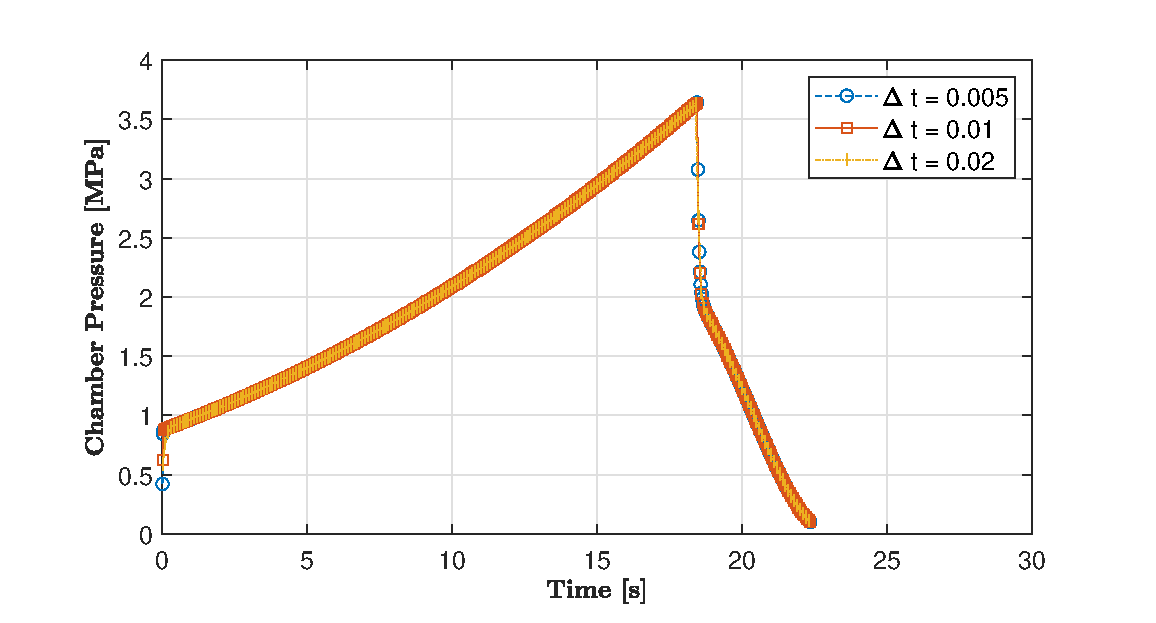
\includegraphics[height = 8.5cm]{graphs/q1_pc.eps}
	\caption{Calculated $p_c$ values using $4^{th}$ order RK method with three different step sizes.}
     \label{fig:q1pc}
\end{figure}

This figure demonstrates how the chamber pressure $p_c$ changes as time progresses. As can be seen in 
Figure \ref{fig:q1pc}, there are three curves, one for each step size. However,
there is no significant difference between the curves, which results from the high degree of accuracy
provided by the $4^{th}$ order RK method. This is because the truncation error for this method is so
small that its effect on the results can be nearly neglected. In addition, using smaller step sizes
helps to calculate more precisely, and it is obvious that the step sizes used for this problem are small
enough. As a result, the values obtained for the chamber pressure $p_c$ of the rocket were approximately
the same for three different step sizes.

\vspace{1em}
Figure \ref{fig:q1rdot} and Figure \ref{fig:q1Isp} demonstrates the change in the rate of equivalent 
radius and the specific impulse with time, respectively.
As it was for $p_c$, there are three curves also for the rate of the equivalent radius
$\dot{r}$ in Figure \ref{fig:q1rdot} and the specific impulse $I_{sp}$ in Figure \ref{fig:q1Isp}. 
Since the conditions are the same as mentioned above, the values calculated for $\dot{r}$ and $I_{sp}$ does not 
experience a major change for different step sizes. The point is, the accuracy of the results obtained by using the RK4 Method
is remarkably of a high degree for the step sizes used in this problem.
\newpage

\begin{figure} [!h]
	\centering
	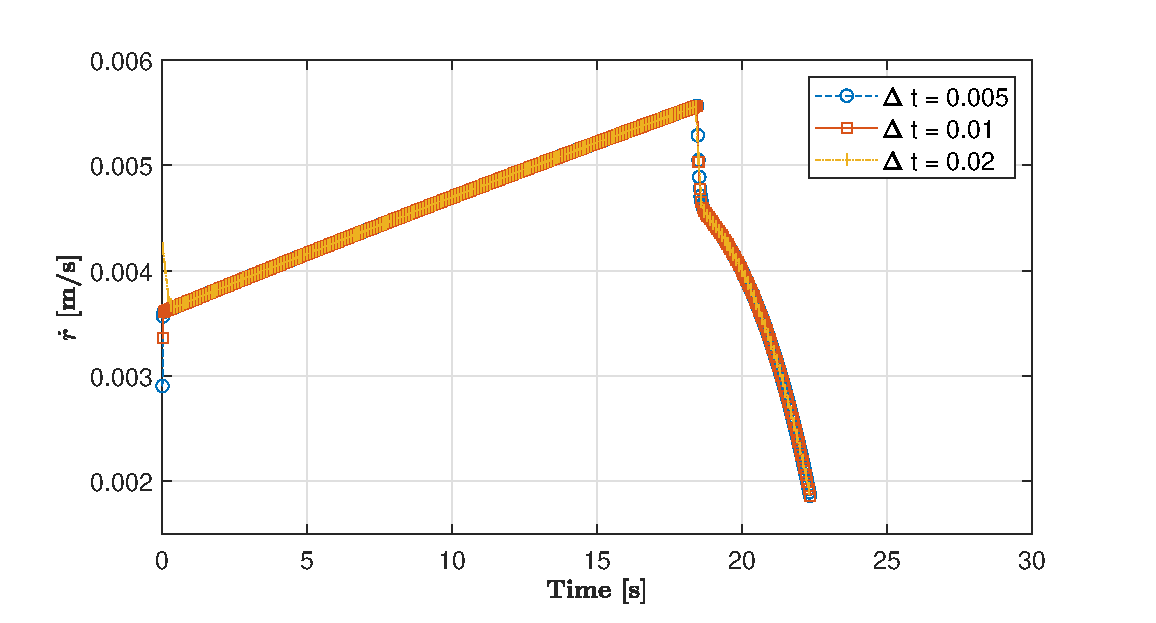
\includegraphics[height = 8.5cm]{graphs/q1_rdot.eps}
	\caption{Calculated $\dot{r}$ values using $4^{th}$ order RK method with three different step sizes.}
	\label{fig:q1rdot}
\end{figure}

\begin{figure} [!h]
	\centering
	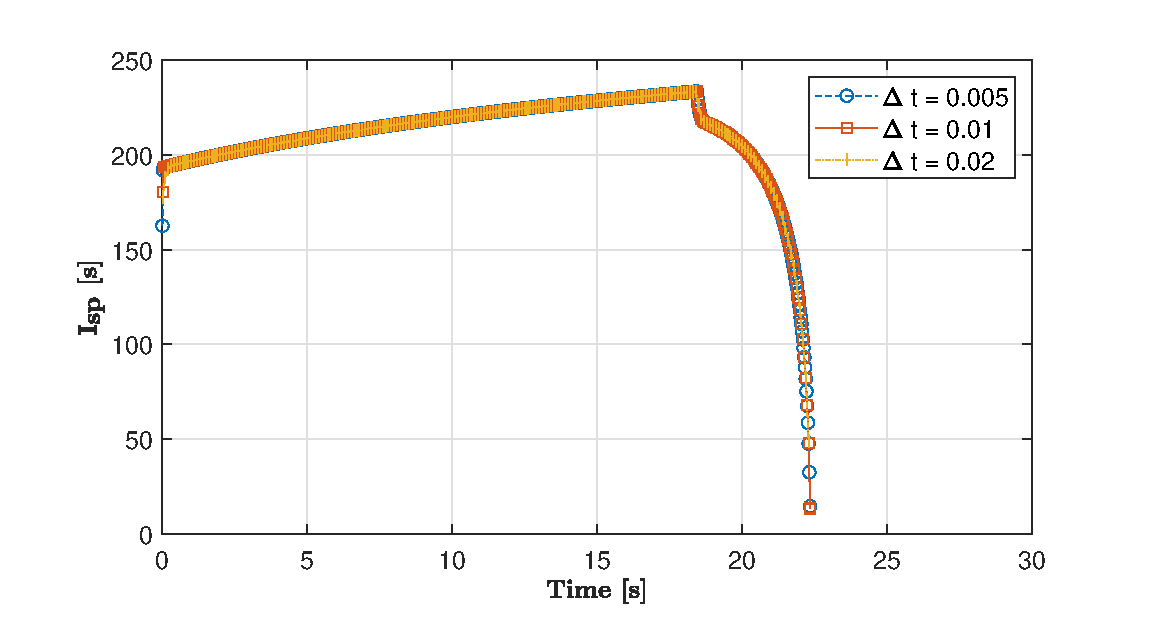
\includegraphics[height = 8.5cm]{graphs/q1_isp.eps}
	\caption{Calculated $I_{sp}$ values using $4^{th}$ order RK method with three different step sizes.}
	\label{fig:q1Isp}
\end{figure}

\newpage

\subsection{Calculation of $p_c$, $\dot{r}$ and $I_{sp}$ with different nozzle throat radiuses}
\begin{figure}[!h]
	\centering
	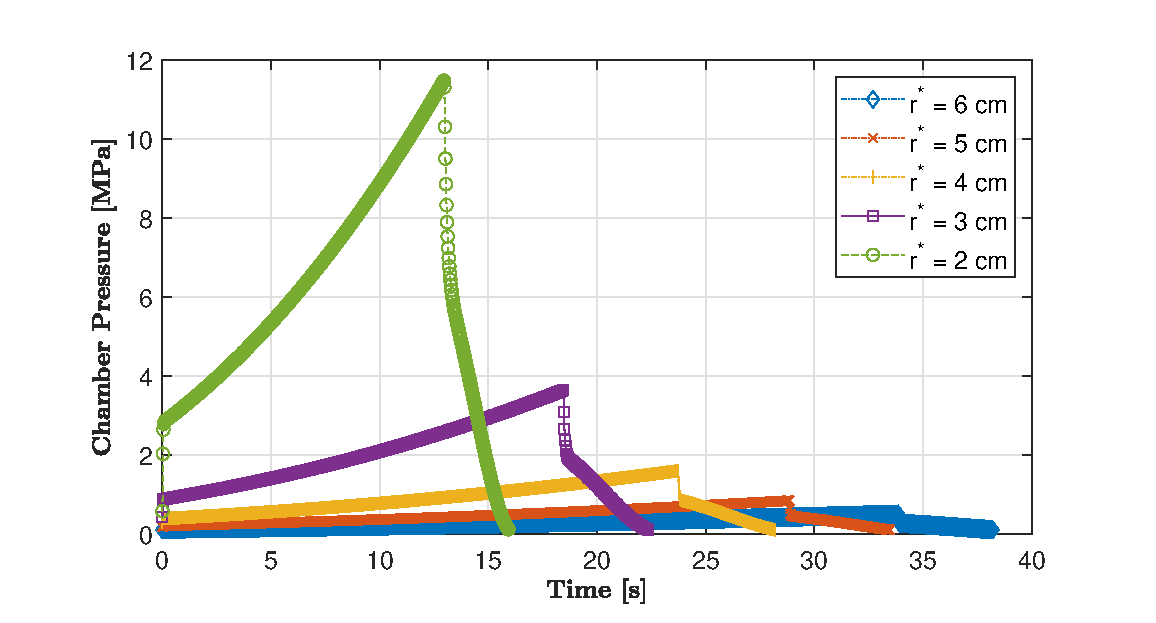
\includegraphics[height = 8.5cm]{graphs/q2_pc.eps}
	\caption{Calculated $p_c$ values using $4^{th}$ order RK method with different nozzle throat radiuses.}
	\label{fig:q2p_cp}
\end{figure}

This figure demonstrates how the chamber pressure $p_c$ changes as time progresses with different nozzle throat radiuses.
As can be concluded from Figure \ref{fig:q2p_cp}, decreasing the radius of the nozzle throat leads to an increase in maximum chamber pressure
and reduces the time needed for the chamber pressure to reach the ambient pressure. 
The reason of this is reducing the radius causes an exponential decrease in the area of the nozzle.
As the area of the nozzle decreases, mass flowing out from the nozzle decreases, and total gas mass inside the cavity increases. 
This results in increased pressure inside the chamber. As the pressure increases, the propellant burns faster. 
Therefore, with a lower nozzle throat radius, propellant depletes faster resulting in shorter flight time.

\newpage
\begin{figure}[!h]
	\centering
	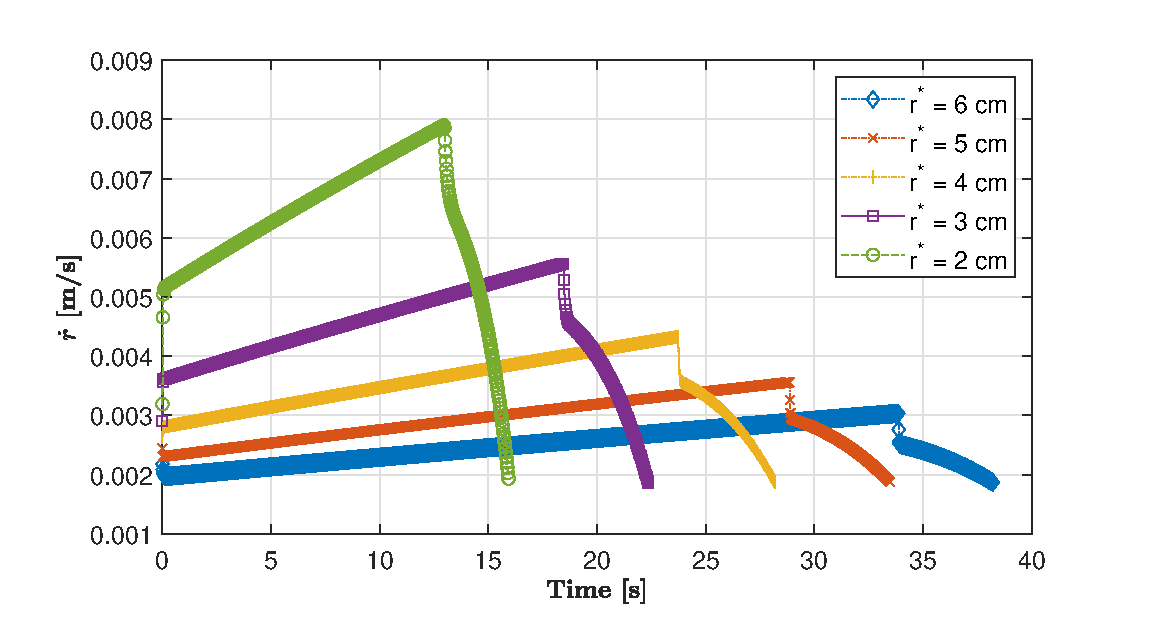
\includegraphics[height = 8.5cm]{graphs/q2_rdot.eps}
	\caption{Calculated $\dot{r}$ values using $4^{th}$ order RK method with different nozzle throat radiuses.}
	\label{fig:q2r_dot}
\end{figure}

This figure illustrates how the burn rate $\dot{r}$ changes as time progresses with different nozzle throat radiuses.
$\dot{r}$ is proportional to $p_c$ as stated in Equation \ref{eqn:pres}; therefore, both of them give 
similar responses to different throat radiuses. 
Lower radiuses cause higher maximum burn rates but shorter time to reach the ambient pressure. 
However, since the propellant burn rate exponent in 
Equation \ref{eqn:pres} is smaller than one, the growth in the maximum burn rates in Figure \ref{fig:q2r_dot} is 
less remarkable than the growth in the maximum chamber pressures in Figure \ref{fig:q2p_cp}. Also, as mentioned above,
flight time decreases because of a faster burn rate.

\newpage

\begin{figure}[!h]
	\centering
	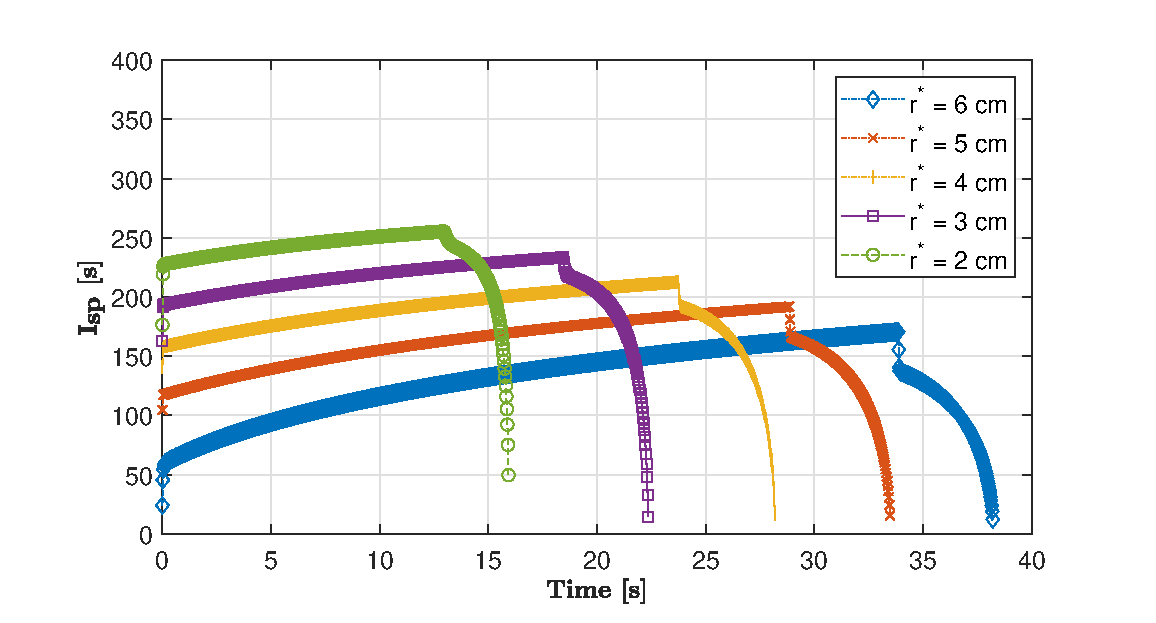
\includegraphics[height = 8.5cm]{graphs/q2_isp.eps}
	\caption{Calculated $I_{sp}$ values using $4^{th}$ order RK method with different nozzle throat radiuses.}
	\label{fig:q2I_sp}
\end{figure}

This figure shows how the specific impulse $I_{sp}$ changes as time progresses with different nozzle throat radiuses.
Specific impulse is a function of chamber pressure $p_c$ as stated in Equation \ref{eq:isp}. 
Therefore, it is not surprising to observe that the specific impulse gives similar reactions in Figure \ref{fig:q2I_sp} 
as the chamber pressure gave in Figure \ref{fig:q2p_cp} in terms of relationship with increasing nozzle throat radius. 
As the radius of the nozzle throat decreases, specific impulse also increases but flight time decreases. Thus, the 
lowest nozzle throat radius of 2 centimeters is the most efficient, as it has the highest specific impulse.

\newpage
\subsection{Calculation of $p_c$, $\dot{r}$ and $I_{sp}$ with adaptive stepping}

\begin{figure}[!h]
	\centering
	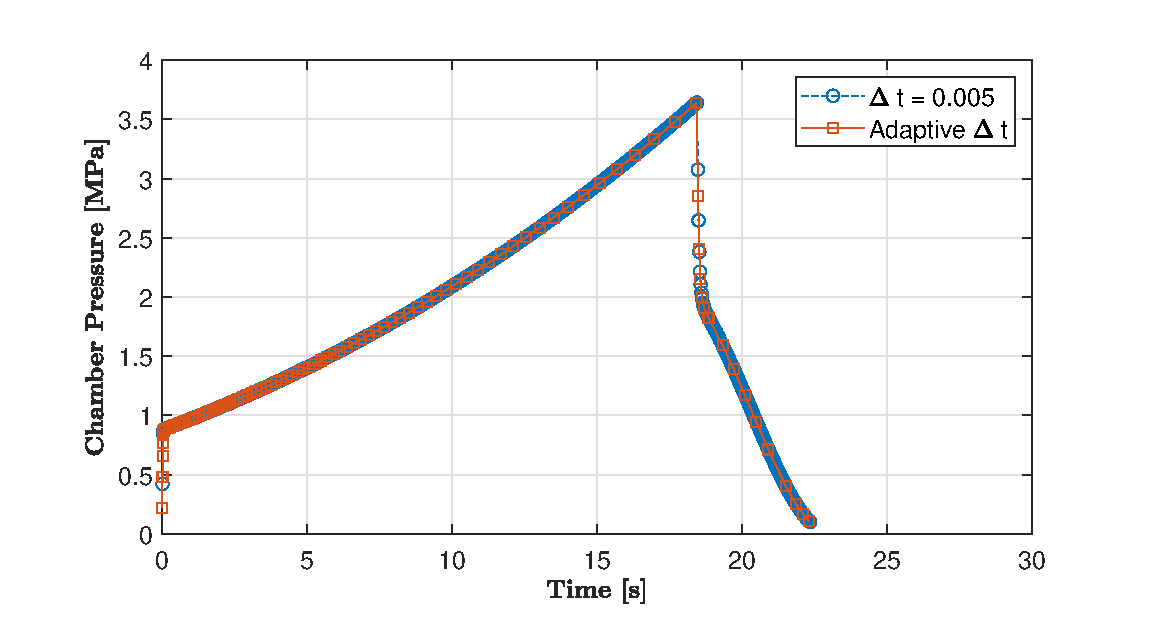
\includegraphics[height = 8.5 cm]{graphs/bonus_pc.eps}
	\caption{Chamber pressure versus time graph with constant and adaptive step size.}
	\label{fig:bonus_cp}
\end{figure}

Figure \ref{fig:bonus_cp}, Figure \ref{fig:bonus_rdot}, and Figure \ref{fig:bonus_isp} illustrate how the chamber pressure, 
the burn rate and specific impulse change as time progresses, respectively, using constant and adaptive time step sizes.
It can be seen from Figures \ref{fig:bonus_cp}, \ref{fig:bonus_rdot}, and \ref{fig:bonus_isp} that when adaptive stepping is 
applied with allowed percent tolerance $E_o = 0.0001$, linear parts can be calculated with fewer steps without losing any accuracy as discussed in 
Section \ref{section:adaptive}. When there is a sudden change, step size gets smaller accordingly and results can be calculated correctly in that region.

It can be seen from Table \ref{tbl:timeint} that using adaptive stepping reduces the total number of time intervals needed significantly.
Although results are calculated three times for each time interval(twice for determining the step size and once for calculating result) 
using the adaptive stepping approach, the number of time intervals needed is much lower than the constant step size approach. Therefore adaptive stepping is 
computationally cheaper without losing accuracy. 


\begin{table}[!h]
	\begin{center}
	\caption{Total number of time intervals needed for computations.}
	\vspace{1em}
	\label{tbl:timeint}
	\begin{tabular}{|c|c|} 
	\hline
	\multicolumn{1}{|c|}{\bf{Stepping Approach}} & \multicolumn{1}{c|}{\bf{Number of time intervals needed}} \\
	\hline
	Constant $\Delta t = 0.005$ &   4470 \\ \hline
	Adaptive Stepping with initial $\Delta t = 0.005$ &   462 \\ \hline
	\end{tabular}
	\end{center}
\end{table}


\newpage

\begin{figure}[!h]
	\centering
	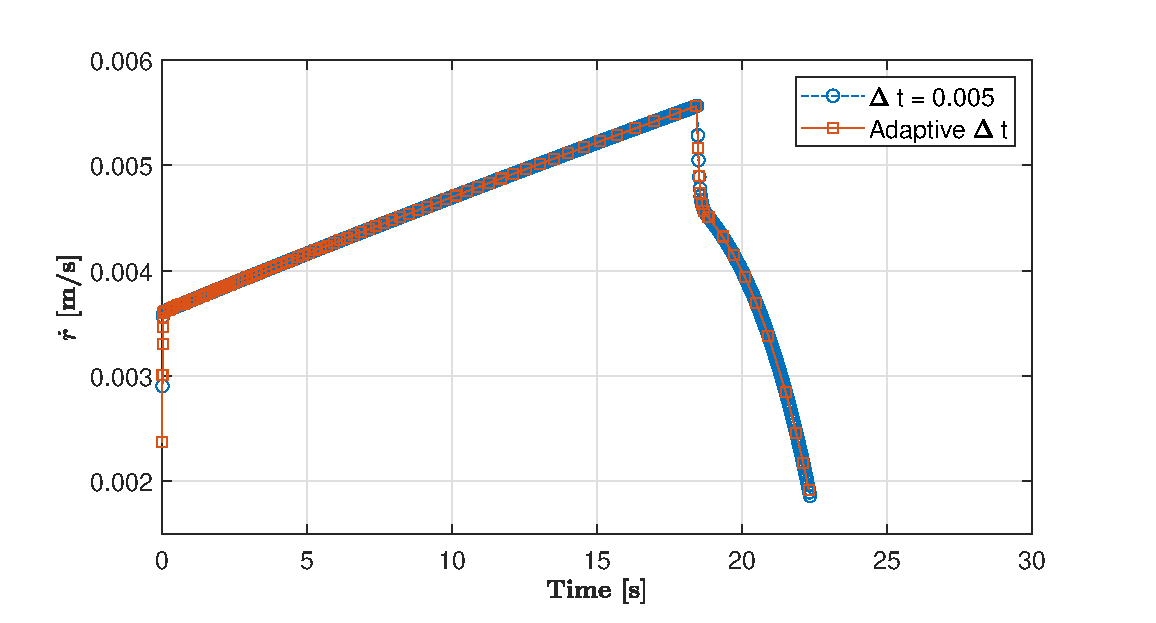
\includegraphics[height = 8.5 cm]{graphs/bonus_rdot.eps}
	\caption{Burn rate versus time graph with constant and adaptive step size.}
	\label{fig:bonus_rdot}
\end{figure}

\begin{figure}[!h]
	\centering
	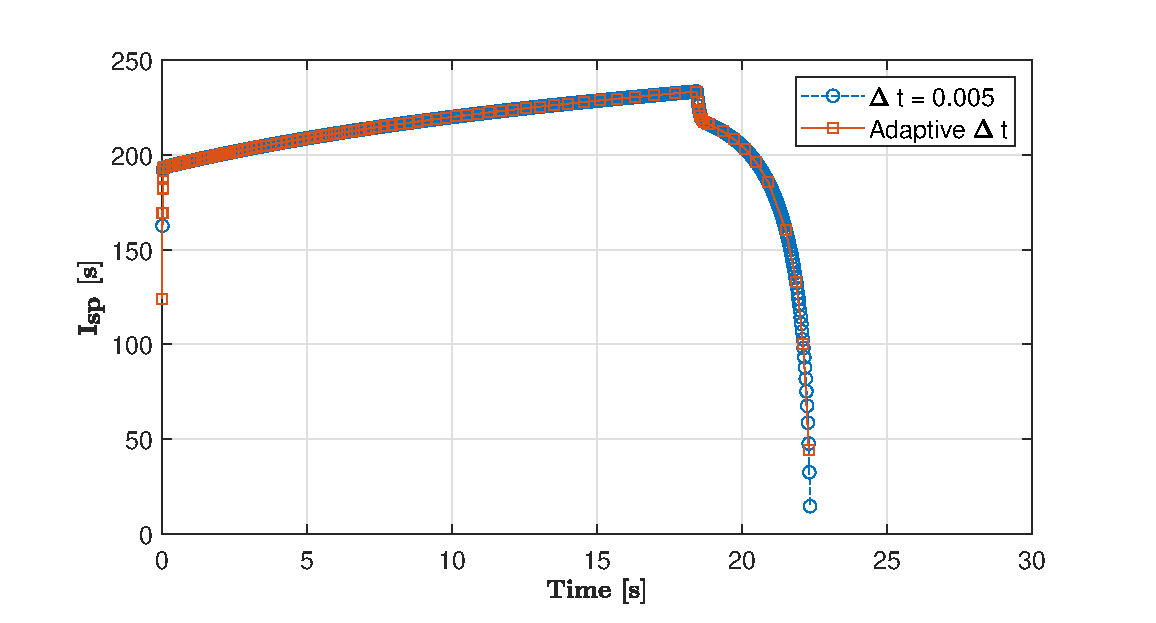
\includegraphics[height = 8.5 cm]{graphs/bonus_isp.eps}
	\caption{Specific impulse versus time graph with constant and adaptive step size.}
	\label{fig:bonus_isp}
\end{figure}

\newpage

\section{Conclusion}

Given a solid-propellant rocket, the change of chamber pressure $p_c$,
the rate of the equivalent radius $\dot{r}$, and the specific impulse $I_{sp}$ were
requested to be calculated in the homework. These calculations were
made by using the classical $4^{th}$ order RK method with three different step sizes for the first
problem, and with different nozzle throat radiuses for the second problem.

At first, comparing the results obtained, it can be observed that the $4^{th}$ order RK method gives
quite reliable results for this problem since the step sizes used are small
enough to give minor error between solutions with different step sizes, and the truncation error
caused by numerical methods is negligible for the $4^{th}$ order RK method. Moving on to the
next comparison, the results illustrate that the outcome of the usage of smaller nozzle throat
radiuses is an increase in maximum chamber pressure. As the burn rate and the specific impulse
are related proportionally to the chamber pressure, their maximum values also experience
an increase. The smaller the nozzle throat radius the harder the gas flows out from the chamber and
the pressure inside the chamber increases, which accounts for the increase in the values
mentioned before.

As a final comment on the problem, it was demonstrated that the effect of adaptive stepping
on the number of time intervals needed is extremely remarkable. It helps to increase
the calculation speed without any loss of accuracy by using a smaller step size for
sudden changes and a bigger step size for linear regions.



\end{document}